
% \begin{figure}[ht]\label{fig:distE}
%   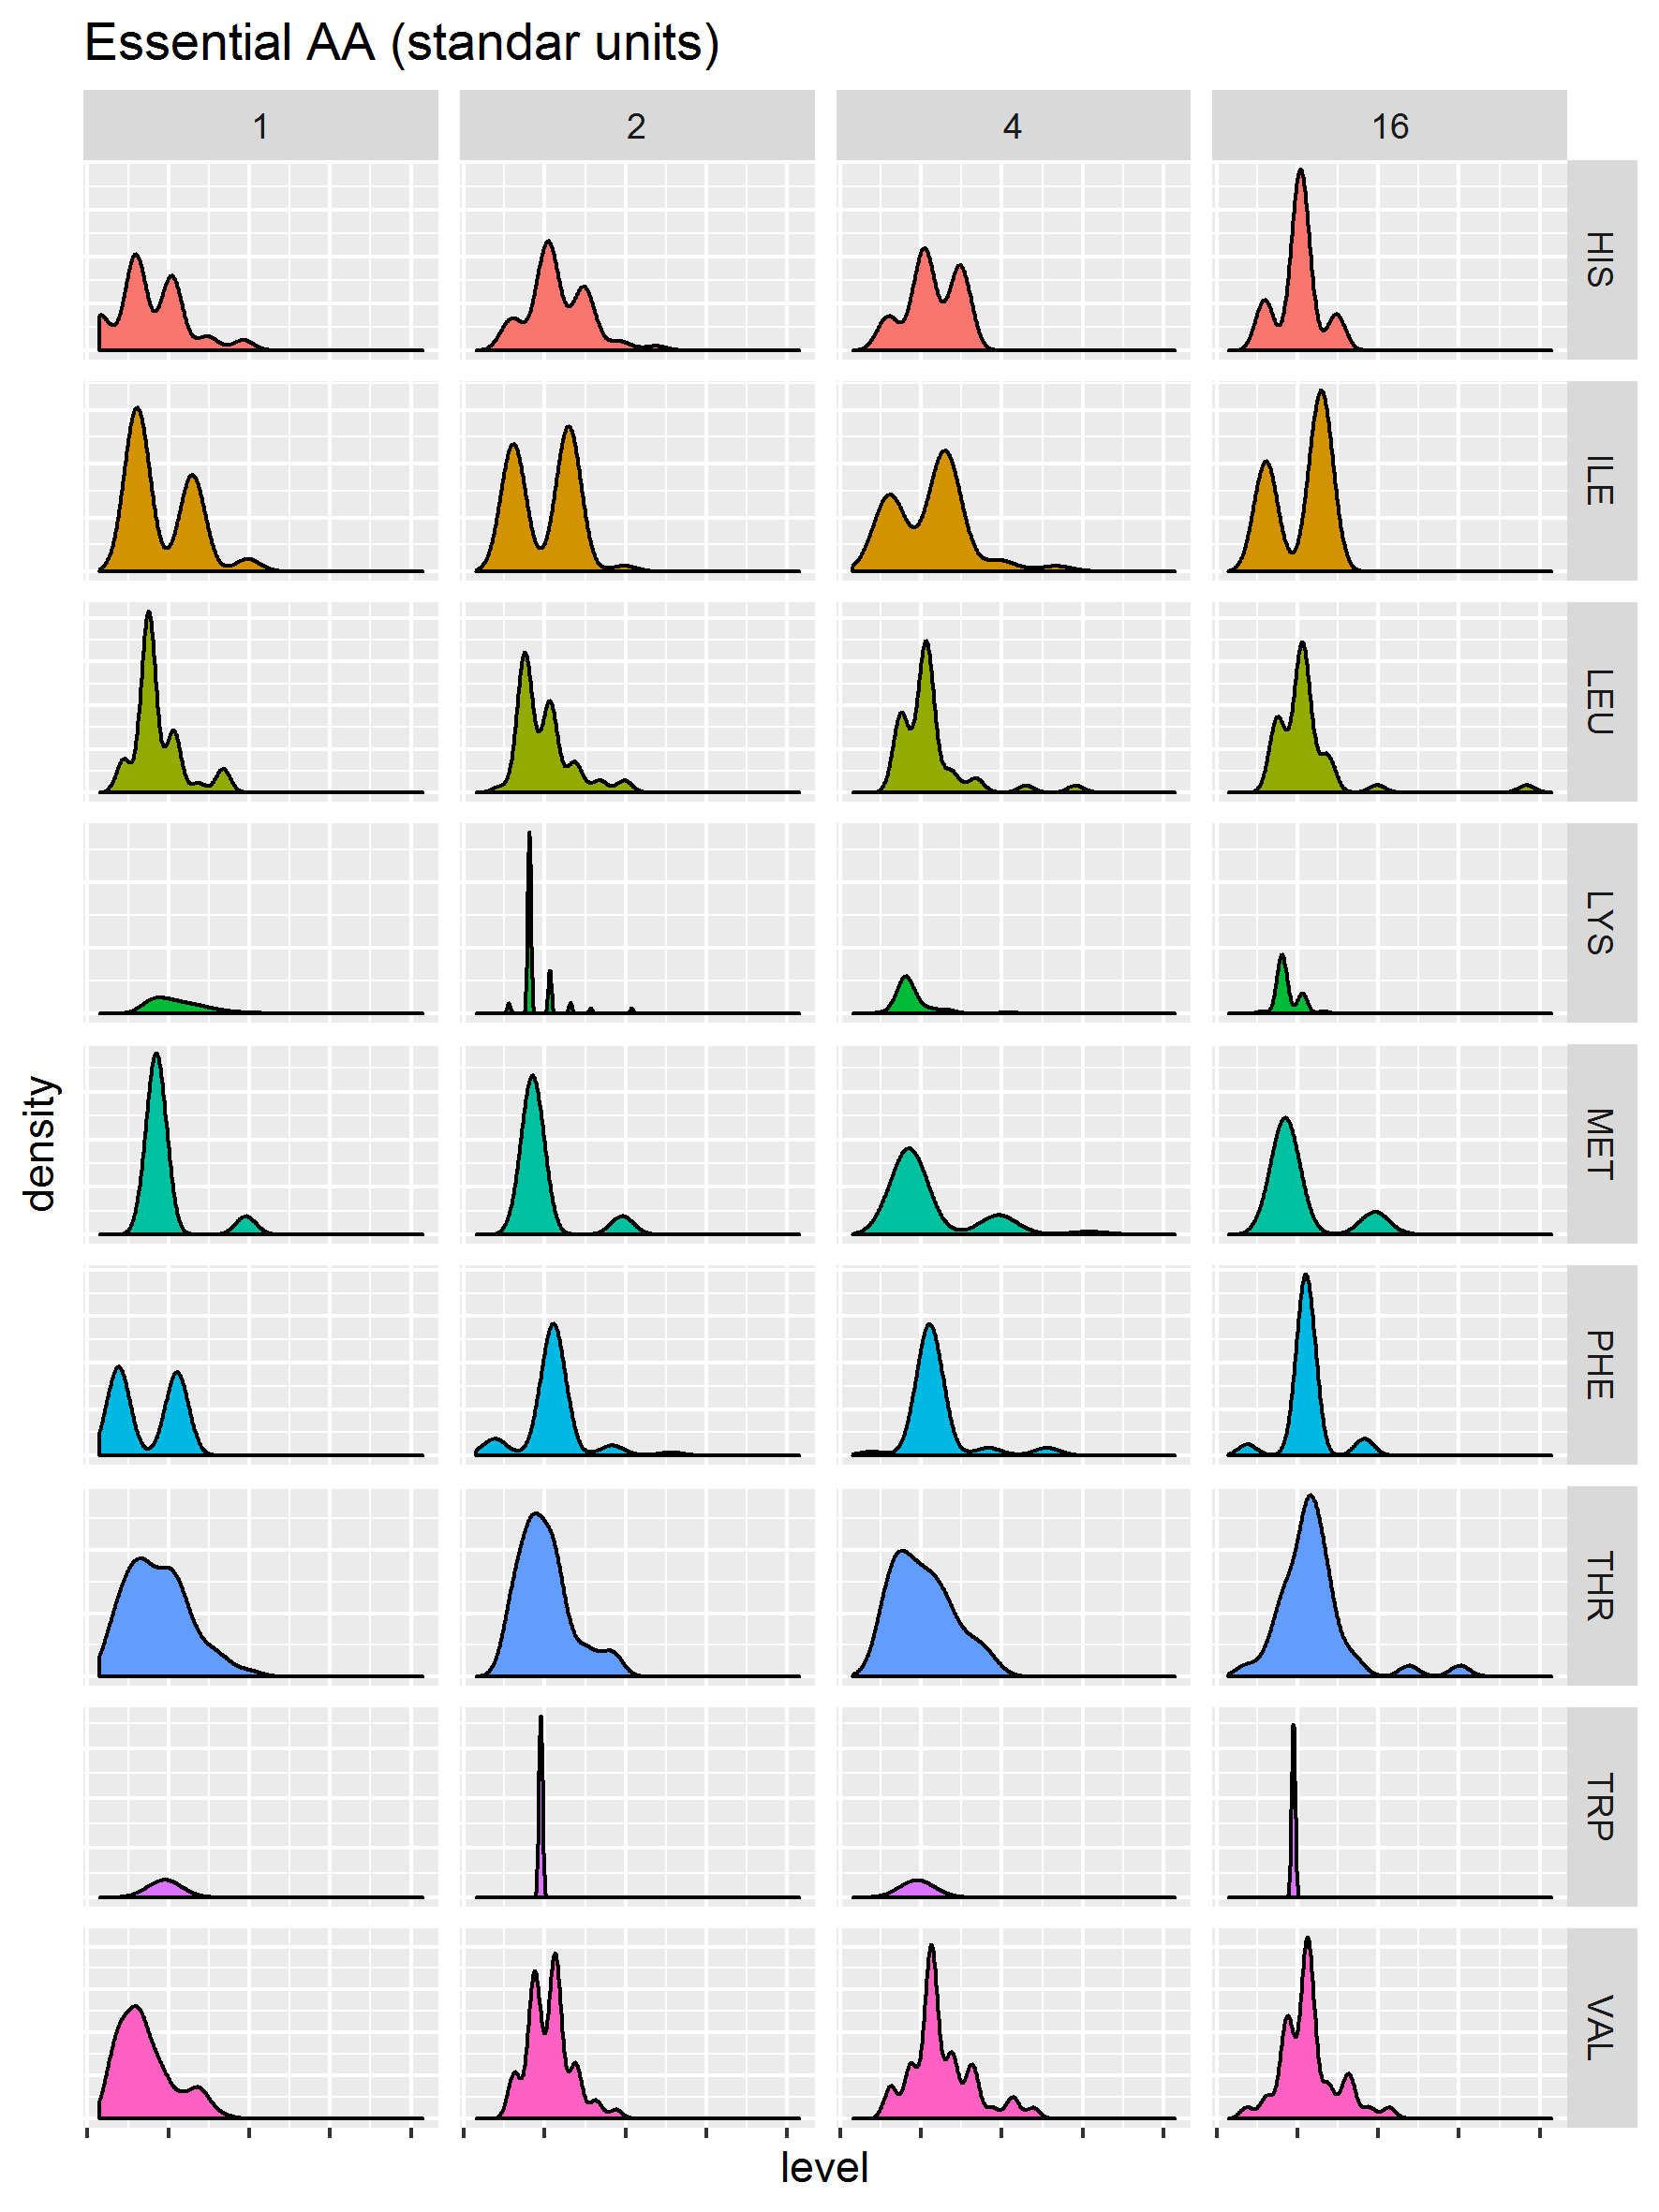
\includegraphics[width=0.9 \textwidth]{../EAA_dist.png}
%   \caption{Distributions of the concentration of Essential AA over time. Each row corresponds to a particular AA. Columns are different weeks. Standard units for the concentratrions are used to make the distributions comparable.}
% \end{figure}
%
%
% \begin{figure}[ht]\label{fig:distNE}
%   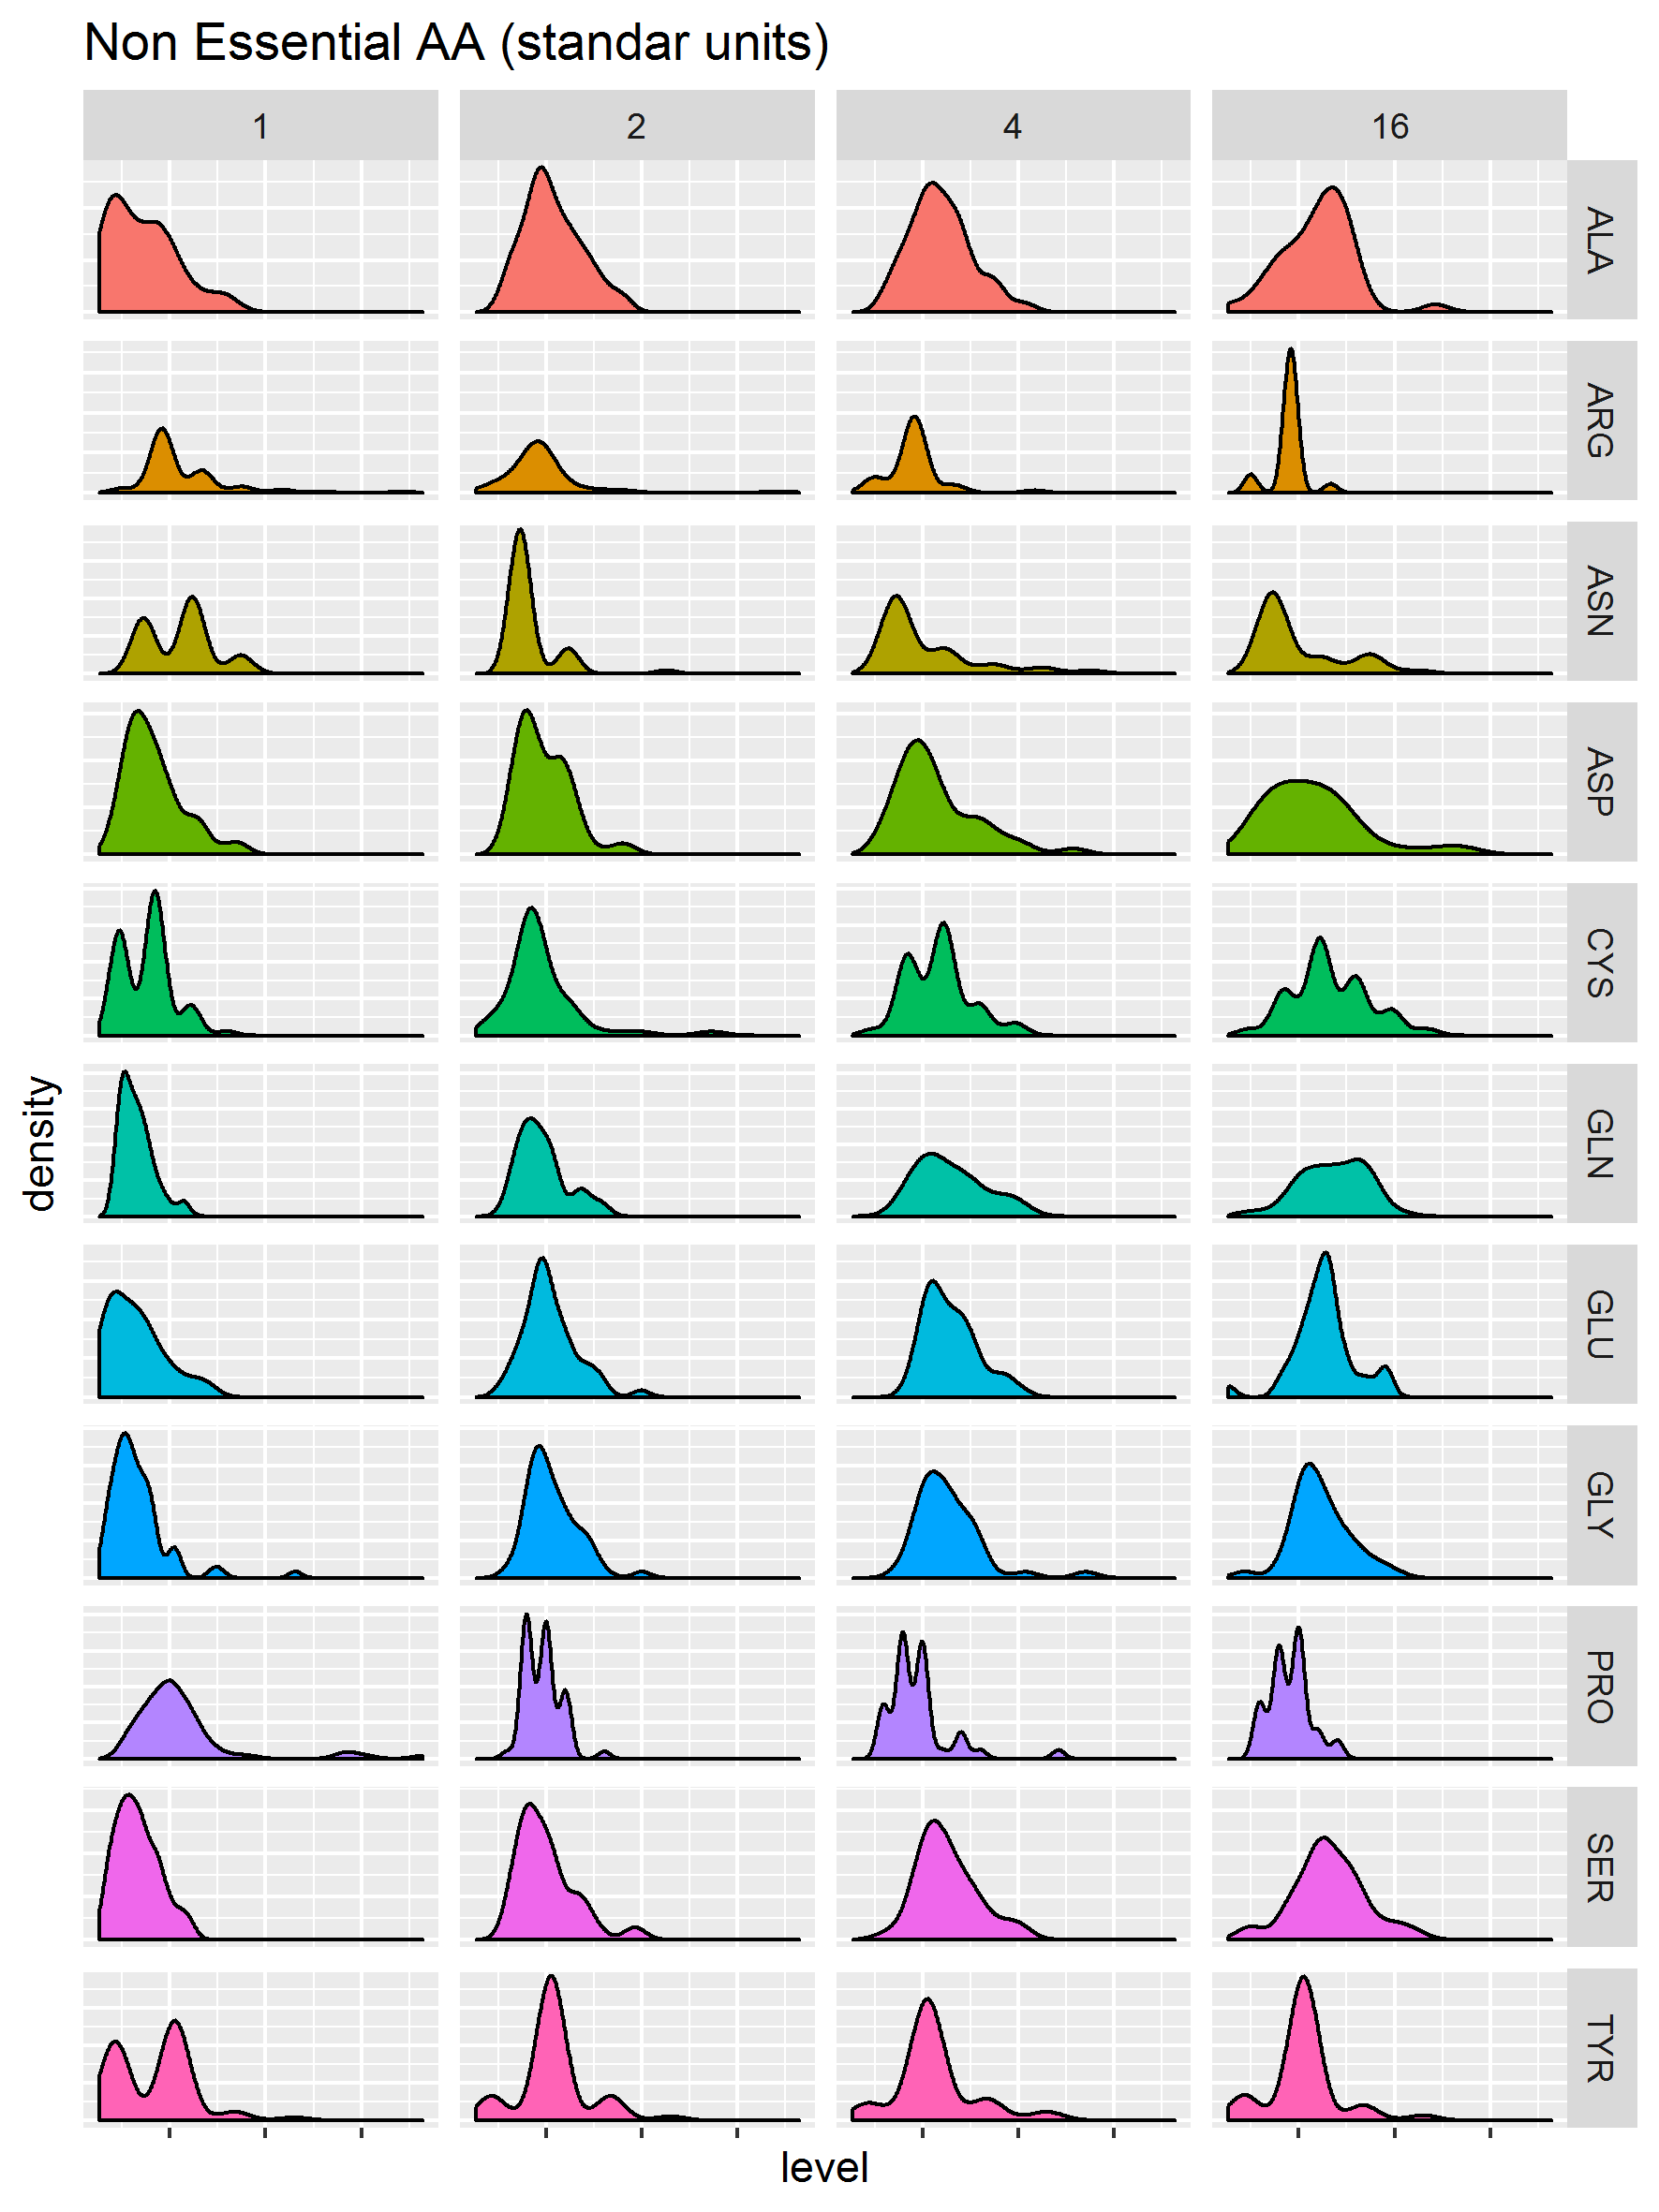
\includegraphics[width=0.9 \textwidth]{../NEAA_dist.png}
%   \caption{Distributions of the concentration of Non Essential AA over time. Each row corresponds to a particular AA. Columns are different weeks. Standard units for the concentratrions are used to make the distributions comparable.}
% \end{figure}


\begin{table}[ht]
  \setlength{\tabcolsep}{12pt}
  \begin{tabular}{cllll}
  AA & \multicolumn{1}{c}{Week 1} & \multicolumn{1}{c}{Week 2} & \multicolumn{1}{c}{Week 4} & \multicolumn{1}{c}{Week 16} \\
  \hline
  \multicolumn{5}{c}{Essential} \\
  \hline
  HIS & 1.43 $\pm$ 0.98 & 2.29 $\pm$ 0.85 & 2.23 $\pm$ 0.71 & 1.95 $\pm$ 0.57 \\
  ILE & 0.45 $\pm$ 0.59 & 0.56 $\pm$ 0.54 & 0.74 $\pm$ 0.68 & 0.62 $\pm$ 0.49 \\
  LEU & 1.38 $\pm$ 1 & 1.79 $\pm$ 1.09 & 2.15 $\pm$ 1.39 & 2.19 $\pm$ 1.7 \\
  LYS & 2.55 $\pm$ 2.21 & 1.38 $\pm$ 0.98 & 1.36 $\pm$ 0.99 & 1.27 $\pm$ 0.56 \\
  MET & 0.09 $\pm$ 0.29 & 0.1 $\pm$ 0.31 & 0.23 $\pm$ 0.48 & 0.16 $\pm$ 0.37 \\
  PHE & 0.48 $\pm$ 0.5 & 1 $\pm$ 0.51 & 1.13 $\pm$ 0.52 & 1.03 $\pm$ 0.37 \\
  THR & 5.08 $\pm$ 3.05 & 6.15 $\pm$ 2.63 & 6.31 $\pm$ 2.9 & 7.68 $\pm$ 3.64 \\
  TRP & 0.03 $\pm$ 0.17 & 0 $\pm$ 0 & 0.03 $\pm$ 0.16 & 0 $\pm$ 0 \\
  VAL & 2.38 $\pm$ 1.34 & 3.73 $\pm$ 1.09 & 4.54 $\pm$ 1.6 & 4.05 $\pm$ 1.39 \\
  \hline
  \multicolumn{5}{c}{Non Essential} \\
  \hline
  ALA & 12.12 $\pm$ 9.02 & 20.98 $\pm$ 7.65 & 24 $\pm$ 8.15 & 24.11 $\pm$ 9.67 \\
  ARG & 1.54 $\pm$ 1.15 & 1.12 $\pm$ 1.06 & 1 $\pm$ 0.69 & 0.95 $\pm$ 0.4 \\
  ASN & 0.75 $\pm$ 0.66 & 0.21 $\pm$ 0.54 & 0.62 $\pm$ 1.02 & 0.54 $\pm$ 0.87 \\
  ASP & 2.66 $\pm$ 2.15 & 3.69 $\pm$ 1.98 & 4.92 $\pm$ 3.06 & 5.03 $\pm$ 3.7 \\
  CYS & 0.77 $\pm$ 0.7 & 1.27 $\pm$ 1.01 & 1.85 $\pm$ 0.87 & 2.3 $\pm$ 1.08 \\
  GLN & 12.6 $\pm$ 10.68 & 31.42 $\pm$ 15.85 & 51.95 $\pm$ 21.76 & 56.05 $\pm$ 21.17 \\
  GLU & 44.92 $\pm$ 33.93 & 89.46 $\pm$ 31.81 & 118.28 $\pm$ 31.19 & 114.84 $\pm$ 35.95 \\
  GLY & 5.03 $\pm$ 4.07 & 10.12 $\pm$ 3.38 & 12.74 $\pm$ 4.46 & 12.24 $\pm$ 3.85 \\
  PRO & 3.6 $\pm$ 2.82 & 2.81 $\pm$ 0.91 & 2.77 $\pm$ 1.68 & 2.54 $\pm$ 1.04 \\
  SER & 4.57 $\pm$ 2.68 & 8.54 $\pm$ 3.62 & 11.62 $\pm$ 3.7 & 12.32 $\pm$ 4.44 \\
  TYR & 0.66 $\pm$ 0.64 & 1.04 $\pm$ 0.58 & 1.13 $\pm$ 0.66 & 1 $\pm$ 0.58 \\
  \hline
  Total	E & 1.54 $\pm$ 2.09	& 1.89 $\pm$ 2.18	& 2.08 $\pm$ 2.36	& 2.11 $\pm$ 2.71 \\
  Total NE	& 8.11  $\pm$ 16.62	& 15.52  $\pm$ 27.51 & 20.99  $\pm$ 36.07	& 21.08  $\pm$ 35.97 \\
  Total	& 5.16 $\pm$ 12.83	& 9.38 $\pm$ 21.54	& 12.48 $\pm$ 28.39	& 12.54 $\pm$ 28.34
  \end{tabular}
  \caption{Free amino acid levels over time.}
\end{table}
